\chapter{Pressure Wave}
\label{sch:pressure_wave}

\section{Introduction}

In laboratory plasma experiments, the profile of the plasma number density is often key to understanding and interpreting the plasma dynamics. Depending on the plasma size and plasma parameters, the plasma density  can typically be inferred through optical diagnostics or through the application of \textit{in situ} diagnostics such as Langmuir probes. In particular, for basic plasma physics experiments, Langmuir probes are commonly used given their simplicity of implementation. Nevertheless, the Langmuir probe measurements require data at multiple probe biases in order for the plasma density to be determined, adding some limitations to their use.  
Furthermore, these probes often only take measurements at a single spatial location, and it can also be challenging to accurately  infer the desired plasma parameters from the probe measurements.
On the other hand, B-dot coils have a simple  conversion from raw measurement to magnetic field values and are used in many devices \cite{Gekelman_Pribyl_Lucky_Drandell_Leneman_Maggs_Vincena_Van_Compernolle_Tripathi_Morales_et_al_2016} \cite{Olson_2020}. Some machines, such as the Big Red Ball (BRB), use arrays of B-dot coils to measure the change in field for each discharge in many spatial locations.

The Terrestrial Reconnection EXperiment (TREX) is a particular configuration implemented in the Big Red Ball (BRB) within the Wisconsin Plasma Physics Laboratory (WiPPL). The configuration is applied to the study of fast magnetic reconnection in a collisionless setting relevant to reconnection in the Earth's magnetosphere. 
The TREX configuration is compatible with  physical diagnostics, and given the relatively large plasma volume, the device is well suited for  the application of both B-dot and Langmuir probes. 

For driving reconnection, TREX applies a strong reconnection drive which includes the sudden energization of a system of coils encircling the plasma. Before the formation of the reconnection current layer, this reconnection drive produces a strong magnetosonic wave including a wave-front moving radially inward towards the center of the device \cite{Olson_Egedal_Clark_Endrizzi_Greess_Millet-Ayala_Myers_Peterson_Wallace_Forest_2021}. The propagation speed of this front is governed by the dispersion relation of the magnetosonic wave, directly related to the plasma density. Below we will discuss and show how the analysis of the wave propagation provides reliable density profiles which are consistent with measurements by Langmuir probes. These profiles characterize the initial plasma produced by an array of plasma guns, which is valuable for analyzing and understanding the plasma dynamics at later times during the plasma discharges.

\subsection{Physical Interpretation}

This wavefront is initialized by a release in magnetic pressure at high radii due to a drop in magnetic field as the drive coils turn on. For plasma near the coils, the magnetic pressure has dropped and thus they are accelerated radially outward. This drops both the plasma pressure and magnetic pressure since the plasma carries the field outwards leading to plasma at lower a radius beginning to expand. This then leads to an iterative process as plasma at lower and lower radii wait until the plasma just above begins to move out.

\section{Observational Evidence}

To induce reconnection in our experiment, we must flip the sign of the reconnecting field, $B_z$. We drive current through the drive coils and in the process of reversing the field and thus forming a reconnection layer, a wavefront in the magnetic field measurements from particle-in-cell simulations and laboratory observations. An example from TREX can be seen in figure \ref{fig:experimental-evolution}.

\begin{figure}
    \centering
    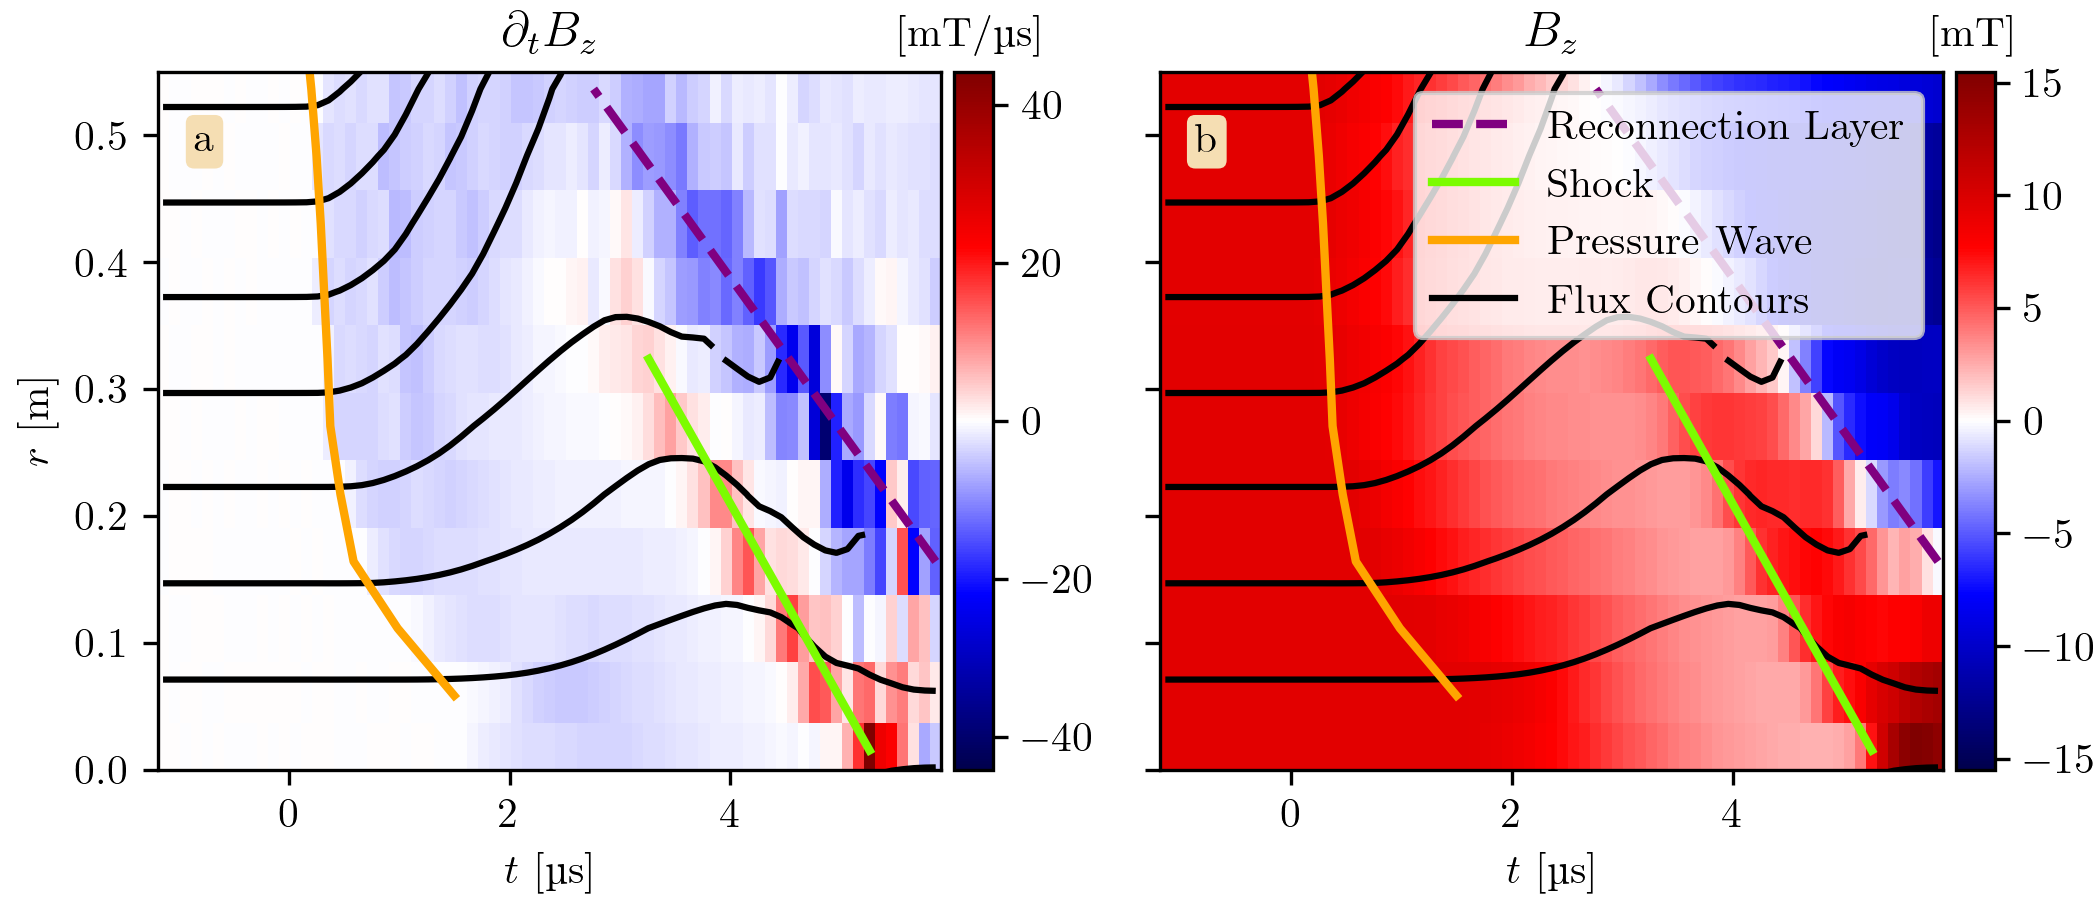
\includegraphics[width=\textwidth]{chapter_pressure_wave/figures/dB_B_and_x_line_shock_pressure_flux.png}
    \caption{Experimental measurements from a single shot where B-dot probes are located along a radial chord at $z=0$. The drive cylinder, at $r = 0.6$ m, starts to reverse the field at $t = 0$. This releases the magnetic pressure at high radii allowing the plasma to expand which leads to a pressure wavefront moving radially inwards (orange). Later, a shock (green) is formed in front of the reconnection layer (purple dashed) which moves radially inwards. Once the pressure wavefront passes, the magnetic field lines start moving outwards following the flux contours (black). The passing of the wavefront leads to a reduction in the initial Helmholtz field before the shock or reconnection layer arrive.}
    \label{fig:experimental-evolution}
\end{figure}

% \subsection{B-dot measurements}

% A common technique in analyzing our data is to measure the radial speed of the reconnection layer by measuring $\partial_t B_z$ as a function of time, $t$, and radius, $r$. This is done by placing probes at many radial positions. As the flux arrays measures the radial profile for multiple $z$ positions, we've taken measurements from a single stick of probes along a radial chord in figure \ref{fig:pressure_wave_speed_probe}.

% \subsubsection{Flux expansion before shock layer}

% Shot 68936 in figure \ref{fig:pressure_wave_speed_probe} shows characteristics that occur in all TREX experiments. This plot is over saturated to highlight salient features. The green line is where the position of the x-point which we can see moves radially inwards (first appearing at around 191 \textmu s). Earlier in time (and lower in radii) is a dark blue region where the sign of $\partial_t B_z$ is opposite of that needed to flip the sign of the magnetic field. This is due to a shock that forms to regulate the reconnection rate (see \cite{Olson_Egedal_Clark_Endrizzi_Greess_Millet-Ayala_Myers_Peterson_Wallace_Forest_2021}).

% The black contours are of constant magnetic flux, which in a cylindrically symmetric system are the paths along which magnetic field lines follow. We see that the field lines begin to move outward far before the reconnection layer passes or the shock compresses them radially inwards. This is a feature of the wave that will help inform our physical understanding of the wave.

\subsubsection{Configuration Dependence}

\begin{figure}
    \centering
    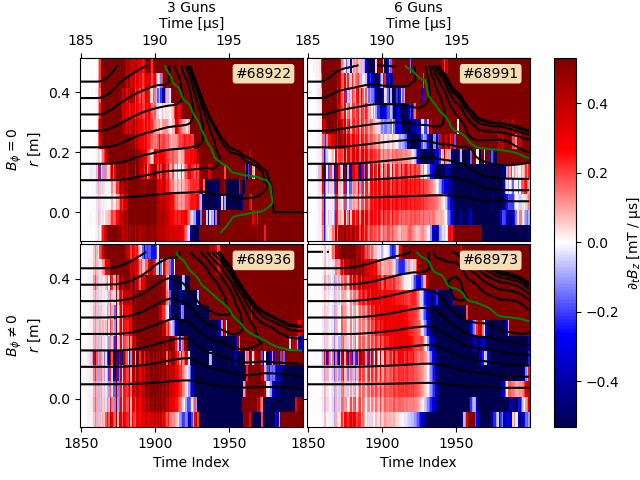
\includegraphics[width=\textwidth]{chapter_pressure_wave/figures/example_speed_probe_panels.png}
    \caption[Pressure Wave Observations in B-dot Measurements]{Measurements of the changing $z$ magnetic field for different configurations. The columns are for three guns and six guns whereas the rows are for zero $\phi$ directed field and non-zero $B_\phi$. The black lines are the flux contours, which in our cylindrically symmetric system are the paths field lines take. The green line is where $B_z = 0$ and thus the approximate radial location of the x-point. Independent of the configuration there is always a brief period where the flux is expanding. The configuration does change the shape of the wavefront though.}
    \label{fig:pressure_wave_speed_probe}
\end{figure}

Each panel in figure \ref{fig:pressure_wave_speed_probe} has a different configuration with the left and right columns being three and six plasma guns respectively (thus changing the total amount of plasma in the machine) and the top and bottom rows having no guide field or having a guide field (thus changing the distribution of the plasma). We find that, independent of background plasma, after the wavefront passes the flux contours begin to move out. This feature travels faster with fewer guns (i.e. getting to a lower radius in a shorter amount of time) and is also a much different shape with and without a guide field.

\subsection{PIC Simulations}

Simulations show very similar results to that of the experiment as can be seen in figure \ref{fig:pressure_wave_greess_simulation}. Here, 2D particle-in-cell simulations of the three coil reconnection experiment show the electron bulk velocity, (d)-(g), and $J_\phi = \partial_z B_r - \partial_r B_z \approx - \partial_r B_z \propto \partial_t B_z$, (h)-(k).

The out of plane current shows the same qualitative features as in figure \ref{fig:pressure_wave_speed_probe} and we see that the electrons drift radially outwards once the wavefront passes, similar to the movement of the magnetic field lines in the experiment.

\subsubsection{Varying Driving Parameters}

Figure \ref{fig:pressure_wave_greess_simulation} shows four configurations of the reconnection experiment where the initial plasma density and peak drive coil current are varied. The shape of the wavefront changes for different densities but does not depend on the driving conditions.

\begin{figure}
    \centering
    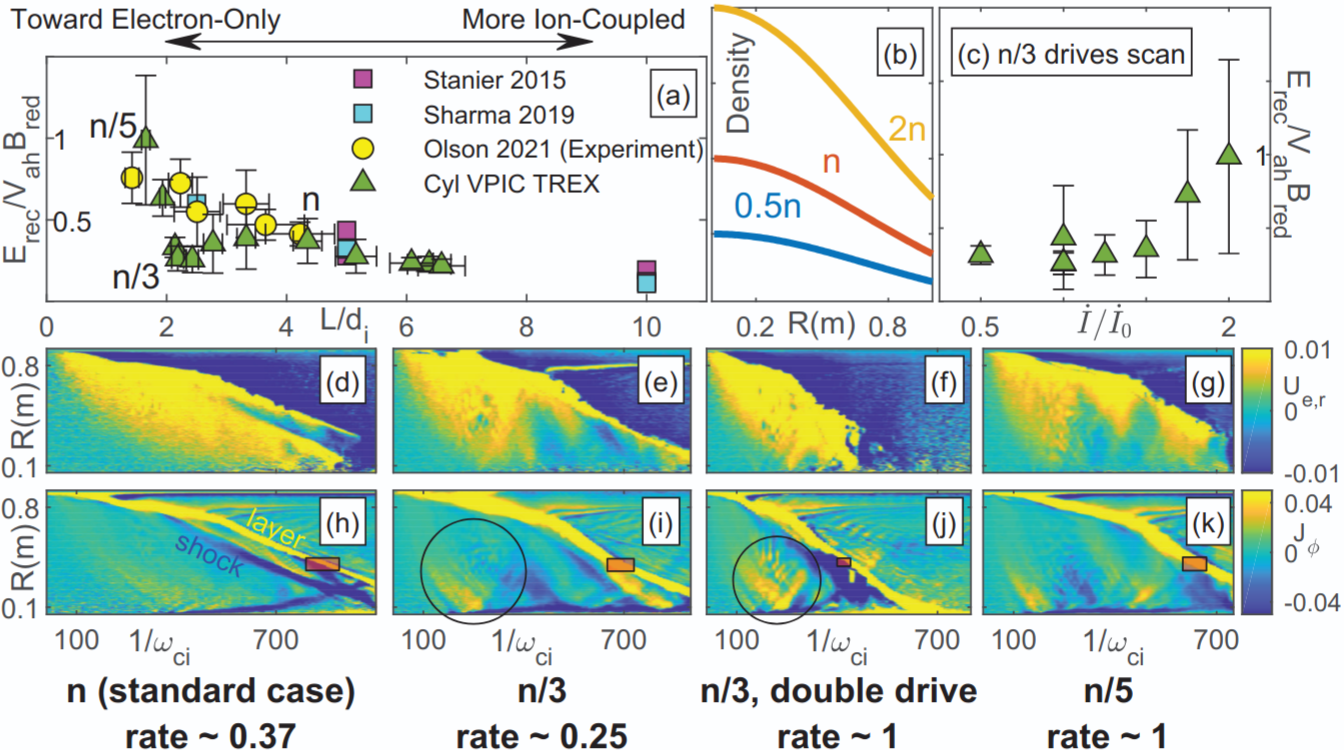
\includegraphics[width=\textwidth]{chapter_pressure_wave/figures/Greess_2022_fig_3.png}
    \caption[Pressure Wave Observations in Simulations]{Reproduction of fig. 3 of \cite{Greess_Egedal_Stanier_Olson_Daughton_Lê_Millet-Ayala_Kuchta_Forest_2022} showing the effect of the pressure wave rebounding off of $R = 0$ and interacting with the reconnection layer. When the rebounding pressure wave hits the layer it can change the reconnection rate which can be seen in panel (a) where there is a dip in the reconnection rate for $n / 3$.}
    \label{fig:pressure_wave_greess_simulation}
\end{figure}

\subsubsection{Changes in Reconnection Rate}

The wavefront moves far faster than both the shock and reconnection layer so does not interact with either on the way towards $r = 0$. Once arriving at the center, the wavefront reflects (black circles in panels (i) and (j) of figure \ref{fig:pressure_wave_greess_simulation}) and depending on when this interaction occurs, can change the reconnection rate (measured in the red rectangle in panels (h)-(k) and plotted as green triangles in panel (a)).

% \section{Physical Interpretation}

% This wavefront is initialized by a release in magnetic pressure at high radii due to a drop in magnetic field as the drive coils turn on. For plasma near the coils, it begins to expand. This drops both the plasma pressure and magnetic pressure since the plasma carries the field radially outwards leading to plasma at lower radius beginning to expand. This then leads to an iterative process as plasma at lower and lower radii wait until the plasma just above begins to move out.

% \subsection{Initial plasma configuration}

% Our system is cylindrically symmetric and plasma is injected from the north pole ($+z$). This plasma then diffuses radially outwards across field lines pointed in either the $z$ direction of the $z$ and $\phi$ directions depending on the use of a guide field. In either case, this can be modeled as a screw pinch equilibrium.

% \subsection{Release in magnetic pressure}

% The drive coils create a field antiparallel to the Helmholtz coil (which creates our initial equilibrium). Since these coils don't ramp up immediately to a high current there is some time when the magnetic pressure near the coils is dropping. The delay in rise is most likely due to transmission line and switch effects that delay the full application of the capacitor bank voltage to the coil leads.

% \subsection{Wavefront as an Information Carrier}



% \subsubsection{Analogous system}

% Sound wave.

% How does a sound wave propagate in a plasma? Fast magnetosonic wave!

% \begin{figure}
%     \caption{Simple diagram of sound wave in container}
% \end{figure}

% \subsection{Modeling magnetic field response}

% \subsubsection{How do we create this model}

% \subsubsection{Pressure wave is like a shield}

% \subsubsection{Example}

% \subsubsection{Why have we mentioned this?}

% \paragraph{Important for probe calibrations}

% \paragraph{Good for predicting effects of different coil configurations}

\section{Wave Simulation}

As we can observe this wavefront in PIC simulations and experimental observations, we will simplify the simulation to linearized MHD. Should this reproduce the features of this wavefront, the core physics of the system can be understood. After the wavefront passes, higher order MHD effects may come into play but that is not of concern to this analysis.

\subsection{Approximations}

For the simulation, we take the following assumptions for simplification:
\begin{itemize}
    \item The toroidal field is unaffected by the plasma. This only matters in cases where we are starting from a screw pinch equilibrium.
    \item The system is cylindrically symmetric.
    \item The plasma can be well modeled by ideal MHD.
\end{itemize}

\subsection{Linearizing MHD}

We start by writing out our conservation laws and Maxwell's equations:
\begin{align}
  \partial_t \rho + \nabla \cdot (\rho \bm{v}) &= 0 \label{eq:mhd_particle_conservation}\\
  \rho \frac{dv}{dt} &= \bm{J} \times \bm{B} - \nabla p \label{eq:mhd_force_balance}\\
  \frac{d}{dt} \left(\frac{p}{\rho^\gamma}\right) &= 0 \label{eq:mhd_energy}\\
  \bm{E} + \bm{v} \times \bm{B} &= 0 \label{eq:mhd_ohms_law}\\
  \nabla \times \bm{E} &= -\partial_t \bm{B} \label{eq:mhd_faradays_law}\\
  \nabla \times \bm{B} &= \mu_0 \bm{J} \label{eq:mhd_amperes_law}\\
  \nabla \cdot \bm{B} &= 0 \label{eq:mhd_div_b}.
\end{align}
We rewrite these equations as the following:
\begin{align}
  \textrm{Eq. }\ref{eq:mhd_force_balance} &\Rightarrow \rho \left( \frac{\partial \bm{v}}{\partial t} + \bm{v} \cdot \nabla \bm{v} \right) = \bm{J} \times \bm{B} - \nabla p \label{eq:mhd_force_balance_simplified}\\
  \textrm{Eq. }\ref{eq:mhd_energy} &\Rightarrow \partial_t p + \bm{v} \cdot \nabla p + \gamma p \nabla \cdot \bm{v} = 0 \label{eq:mhd_energy_simplified}\\
  \textrm{Eq. }\ref{eq:mhd_ohms_law} + \ref{eq:mhd_faradays_law} &\Rightarrow \frac{\partial \bm{B}}{\partial t} = \nabla \times (\bm{v} \times \bm{B}) \label{eq:mhd_ohms_faradays_simplified}.
\end{align}
Then we expand around equilibrium assuming each variable can be written as $X = X_0 + X_1(t)$ where $X_0$ is the equilibrium value and $X_1$ is a perturbation. We'll assume that the equilibrium values are constant in time and that the perturbations are small. Thus,
\begin{align}
    \textrm{Eq. } \ref{eq:mhd_particle_conservation} &\Rightarrow \frac{\partial \rho_1}{\partial t} = - \nabla \cdot (\rho_0 \bm{v_1}) \label{eq:mhd_particle_linear}\\
    \textrm{Eq. } \ref{eq:mhd_force_balance_simplified}, \ref{eq:mhd_amperes_law} &\Rightarrow \rho_0 \frac{\partial \bm{v_1}}{\partial t} = \frac{1}{\mu_0} ((\nabla \times \bm{B}_1) \times \bm{B}_0 + (\nabla \times \bm{B}_0) \times \bm{B}_1) - \nabla p_0 - \nabla p_1 \label{eq:mhd_force_balance_linear}\\
    \textrm{Eq. } \ref{eq:mhd_energy_simplified} &\Rightarrow \frac{\partial p_1}{\partial t} = -\bm{v_1} \cdot \nabla p_0 -\gamma p_0 \nabla \cdot \bm{v_1} \label{eq:mhd_energy_linear}\\
    \textrm{Eq. } \ref{eq:mhd_ohms_faradays_simplified} &\Rightarrow \frac{\partial \bm{B}_1}{\partial t} = \nabla \times (\bm{v_1} \times \bm{B}_0) \label{eq:mhd_ohms_faradays_linear}.
\end{align}
Let $\bm{\xi}$ be a displacement vector that represents the perturbation and thus $\partial_t \bm{\xi} = \bm{v}_1$. By dropping higher order terms we find
\begin{align}
  \textrm{Eq. } \ref{eq:mhd_particle_linear} &\Rightarrow \partial_t \rho_1 = - \nabla \cdot (\rho_0 \partial_t \bm{\xi}) \nonumber \\
  &\Rightarrow \rho_1 = - \nabla \cdot (\rho_0 \bm{\xi}) \label{eq:mhd_particle_linear_displacement}\\
  \textrm{Eq. } \ref{eq:mhd_force_balance_linear} &\Rightarrow \rho_0 \partial_{tt} \bm{\xi} = \frac{1}{\mu_0} ((\nabla \times \bm{B}_1) \times \bm{B}_0 + (\nabla \times \bm{B}_0) \times \bm{B}_1) - \nabla p_0 - \nabla p_1 \label{eq:mhd_force_balance_linear_displacement}\\
  \textrm{Eq. } \ref{eq:mhd_energy_simplified} &\Rightarrow \partial_t p_1 = -\partial_t \bm{\xi} \cdot \nabla p_0 -\gamma p_0 \nabla \cdot \partial_t \bm{\xi} \nonumber \\
  &\Rightarrow p_1 = -\bm{\xi} \cdot \nabla p_0 -\gamma p_0 \nabla \cdot \bm{\xi} \label{eq:mhd_energy_linear_displacement}\\
  \textrm{Eq. } \ref{eq:mhd_ohms_faradays_linear} &\Rightarrow \partial_t \bm{B}_1 = \nabla \times (\partial_t \bm{\xi} \times \bm{B}_0) \nonumber \\ 
  &\Rightarrow \bm{B}_1 = \nabla \times (\bm{\xi} \times \bm{B}_0) \label{eq:mhd_ohms_faradays_linear_displacement}.
\end{align}

By combining \ref{eq:mhd_force_balance_linear_displacement}, \ref{eq:mhd_energy_linear_displacement}, and \ref{eq:mhd_ohms_faradays_linear_displacement}, we can write a first-order perturbation expansion of the plasma as
\begin{align}
  \rho_0 \partial_{tt} \bm{\xi} =& \frac{1}{\mu_0}\left\{\nabla \times \left[\nabla \times \left(\bm{\xi} \times \bm{B}_0\right)\right]\right\}\times \bm{B}_0 + \frac{1}{\mu_0} \left(\nabla \times \bm{B}_0\right) \times \left[\nabla \times \left(\bm{\xi} \times \bm{B}_0\right)\right] \nonumber \\
  &- \nabla p_0 + \nabla \left(\bm{\xi} \cdot \nabla p_0 + \gamma p_0 \nabla \cdot \bm{\xi}\right)
  \label{eq:first_order_mhd}
\end{align}
This gives us three equations which we can apply the systems symmetries to for further simplification.

\subsection{Plasma Equilibrium + Symmetries}

\subsubsection{Types of Equilibrium}

Our experimental system evolves to an equilibrium as the plasma is injected into the machine along flux tubes. As the ions have a gyroradius on the order of a centimeter, these flux tubes are very thin but the plasma begins to diffuse across field lines in both the toroidal and radial directions leading to a toroidally symmetric and radially decreasing density profile.

\paragraph{\texorpdfstring{$\theta$}{Theta}-pinch}

If the only initial field is due to the Helmholtz coil, the plasma pressure is only balanced by a $z$ directed magnetic field thus giving a $\theta$-pinch equilibrium defined by \cite{Freidberg_2014}
\begin{equation}
    p + \frac{B_z^2}{2\mu_0} = \frac{B_0^2}{2 \mu_0}.
    \label{eq:theta_pinch_equilibrium}
\end{equation}
% See \cite{Freidberg_2014} for a derivation of this (section 5.2) and the screw pinch equilibrium (section 5.4).

\paragraph{Screw-pinch}

With a guide field, the system changes as we now have a toroidal field that goes like
\begin{equation}
    B_\phi(r) = \frac{\mu_0 I}{2 \pi r}.
\end{equation}
The plasma could potentially perturb this toroidal field and we lack a measurement of the static magnetic field. Luckily, a perturbation of this field would require a plasma current in the $z$-direction and since the permanent magnets confine the plasma in the axial direction, any net current would be small.

Our screw-pinch equilibrium is \cite{Freidberg_2014}
\begin{equation}
    \dv{r} \left(p + \frac{B_z^2 + B_\phi^2}{2 \mu_0}\right) + \frac{B_\phi^2}{2 \mu_0} = 0.
    \label{eq:screw_pinch_equilibrium}
\end{equation}
If the toroidal field is unperturbed from it's vacuum value, this reverts back to the $\theta$-pinch equilibrium which we'll use in the simulation.

\subsubsection{Types of Symmetries}

We now discuss the validity of our symmetry assumptions that were made initially and we will use for further simplification of the linearized MHD equation.

% \paragraph{Z-symmetry}

It can be seen that along the equator of the machine, and as previously discussed, everything about our system is mirror symmetric except the plasma guns. Since the thermal speed if far larger than the diffusion speed we can assume $z$ symmetry from the guns. Additionally, the magnetic field from the Helmholtz coil is nearly uniform along the $z$ direction and the magnetic field from the coils is symmetric near the $z$-center of the coil system (edge effects cause $r$ directed fields thus removing $z$ translational symmetry because of $\nabla \cdot \vb{B} = 0$). Our simulation and measurements are only done at the mean $z$ of the coils to minimize these effects.

% \paragraph{\texorpdfstring{$\phi$}{Phi}-symmetry}

In the $\phi$ direction, we lack symmetry at two locations. The guns inject in a hexagonal pattern or symmetric subgroups of that at a radius of approximately 10 cm. Although the distance between guns when we are only using three guns is approximately 20 cm meaning that toroidal isotropization is on that length scale, we find through measurements that the plasma has toroidal symmetry. The second source of asymmetry is due to the drive coil leads. Since the leads are close together and in the drive cylinder case, are well shielded, we can ignore this effect as long as we are far from the drive coil radii.

\subsection{Simplified 1D equation}

We assume that the perturbation only depends on $r$ since we are symmetric in $\phi$ and $z$. Thus we can write $\bm{\xi}$ as
\begin{equation*}
  \bm{\xi} = \xi_r(r) \hat{r} + \xi_\phi(r) \hat{\phi} + \xi_z(r) \hat{z} \label{eq:xi_vector}
\end{equation*}
Using equation \ref{eq:screw_pinch_equilibrium} and assuming that the toroidal field is not affected by the plasma we get
\begin{align}
  B_{\phi, 0} &= \frac{\mu_0 I_\mathrm{TF}}{2 \pi r} \label{eq:toroidal_field} \\
  \Rightarrow \partial_r p_0 &= -\frac{1}{\mu_0} \left( B_{\phi, 0} \partial_r B_{\phi, 0} + B_{z, 0} \partial_r B_{z, 0} + \frac{B_{\phi, 0}^2}{r} \right) \\
  &= -\frac{1}{\mu_0} B_{z, 0} \partial_r B_{z, 0} \label{eq:simple_screw_pinch_pressure_gradient}.
\end{align}
This is the same as the $\theta$-pinch equilibrium (equation \ref{eq:theta_pinch_equilibrium}). Integrating we find
\begin{equation}
  p_0 + \frac{B_{z, 0}^2}{2 \mu_0} = C \label{eq:screw_pinch_equilibrium_integrated},
\end{equation}
where $C$ is a constant. Assuming the plasma displaces the initial vacuum field as it enters the machine we let $C = B_H^2 / 2 \mu_0$ where $B_H$ is the Helmholtz field. Here we have assumed the pressure stays constant from before plasma to after. Physically this is not the case because the outward pressure of the plasma bends the field lines causing additional magnetic pressure but this effect is small. Since the Helmholtz changes as a small amount as a function of radius, we set $B_H$ to be the vacuum field strength at $r = 0$.

Solving for the pressure from equation \ref{eq:screw_pinch_equilibrium_integrated} we find
\begin{align*}
  \rho_0(r) \partial_{tt} \xi_r &= \frac{1}{2 \mu_0 r^2} \bigg[ r^2 \xi_r''(r) \left(\frac{5 B_H^2}{3}+2 B_{\phi, 0}(r)^2+\frac{B_{z,0}(r)^2}{3}\right) \\
  & + r \xi_r'(r) \bigg(\frac{5 B_H^2}{3}+6 r B_{\phi, 0}(r) B_{\phi, 0}'(r)+4 B_{\phi, 0}(r)^2 \\
  &\qquad \qquad +\frac{1}{3} B_{z,0}(r) \left(2 r B_{z,0}'(r)+B_{z,0}(r)\right)\bigg) \\
  & + \xi_r(r) \bigg(-\frac{5 B_H^2}{3}+2 r^2 B_{\phi, 0}(r) B_{\phi, 0}''(r) \\
  & \qquad \qquad +2 r B_{\phi, 0}'(r) \left(r B_{\phi, 0}'(r)+2 B_{\phi, 0}(r)\right) \\
  & \qquad \qquad -\frac{1}{3} B_{z,0}(r) \left(B_{z,0}(r)-2 r B_{z,0}'(r)\right)\bigg) \bigg], \\
  \partial_{tt} \xi_\phi &= 0, \\
  \partial_{tt} \xi_z &= 0,
\end{align*}
where $\gamma = 5/3$. Since the second derivative is zero in both the $\phi$ and $z$ directions this means the wave only perturbs the plasma radially, as expected for an expanding plasma. We rewrite the density in terms of other values such that our only simulation inputs are the electron temperature, number density profile, background $z$ and $\phi$ fields, and particle masses.
\begin{align*}
  p_0(r) &= T_0 n_0(r) = \frac{1}{2 \mu_0}(B_H^2 - B_{z0}(r)^2) = T_0 \frac{\rho_0(r)}{m_i + m_e} \\
  \Rightarrow \rho_0(r) &= \frac{m_i + m_e}{2 T_0 \mu_0}(B_H^2 - B_{z0}(r)^2)
\end{align*}
In our experiment, the ion temperature is far smaller than the electron temperature and thus $p = n T_e$.

\subsubsection{Equation Interpretation}

We can see that equation \ref{eq:dedimensionalized_pde} looks something like a wave equation with the form
\begin{equation*}
    \partial_{tt} \xi = D \partial_{rr} \xi
\end{equation*}
where $D > 0$ and we have dropped the subscript on $\xi_r$. The various terms with $r$ act in a geometric fashion as the wave travels towards low radii and the magnetic field acts to change the wave speed. This isn't immediately obvious but will be seen in simulation outputs.

\subsubsection{Normalized equation}

We nondimensionalize our equation such that it can be simulated numerically. Let $r = \tilde{r}R$, $B = \tilde{B}B_H$, $t=t_0 \tau$. Thus $\partial_r = 1/R \partial_{\tilde{r}}$, $\partial_t = 1/t_0 \partial_\tau$, and $\xi = \tilde{\xi}R$. We'll now use primes to denote derivatives in $\tilde{r}$. Thus we have
\begin{align}
  % \partial_{\tau\tau}\tilde{\xi} =& \underbrace{\frac{T_0 t_0^2}{3 R^2 (m_i + m_e)}}_{C} \frac{1}{\tilde{r}^2\left(1 - \tilde{B}_{z0}(\tilde{r})^2\right)} \left[-\tilde{\xi} \left(5 + \tilde{B}_{z0}^2 - 2 \tilde{r} \tilde{B}_{z0}\tilde{B}_{z0}'\right) + \tilde{r}\tilde{\xi}' \left(5 + \tilde{B}_{z0}^2 + 2 \tilde{r} \tilde{B}_{z0}\tilde{B}_{z0}'\right)+\tilde{r}^2 \tilde{\xi}'' \left(5 + \tilde{B}_{z0}^2\right)\right]
  \partial_{\tau\tau}\tilde{\xi} =& \underbrace{\frac{T_0 t_0^2}{3 R^2 (m_i + m_e)}}_{C} \frac{1}{\tilde{r}^2\left(1 - \tilde{B}_{z, 0}(\tilde{r})^2\right)} \left[ A(\tilde{r}) \tilde{r}^2 \tilde{\xi}'' + B(r) \tilde{r}\tilde{\xi}' + C(\tilde{r}) \tilde{\xi} \right]
  \label{eq:dedimensionalized_pde} \\
  A(\tilde{r}) =& 5 + 6 \tilde{B}_{\phi, 0}(r)^2 + \tilde{B}_{z, 0}(\tilde{r})^2 \nonumber \\
  B(\tilde{r}) =& 5 + 18 \tilde{r} \tilde{B}_{\phi, 0}(\tilde{r}) \tilde{B}_{\phi, 0}'(\tilde{r}) + 12 \tilde{B}_{\phi, 0}(\tilde{r})^2 + \tilde{B}_{z, 0}(\tilde{r}) \left(2 \tilde{r} \tilde{B}_{z, 0}'(\tilde{r}) + \tilde{B}_{z, 0}(\tilde{r})\right) \nonumber \\
  C(\tilde{r}) =& -5 + 6 \tilde{r}^2 \tilde{B}_{\phi, 0}(\tilde{r}) \tilde{B}_{\phi, 0}''(\tilde{r}) + 6 \tilde{r} \tilde{B}_{\phi, 0}'(\tilde{r}) \left(\tilde{r} \tilde{B}_{\phi, 0}'(\tilde{r}) + 2 \tilde{B}_{\phi, 0}(\tilde{r})\right) \nonumber \\
  &- \tilde{B}_{z, 0}(\tilde{r}) \left(\tilde{B}_{z, 0}(\tilde{r}) - 2 \tilde{r} \tilde{B}_{z, 0}'(\tilde{r})\right) \nonumber.
\end{align}
The first fraction is made of constants and we'll call the first coefficient $C$. By choosing a value for $C$ we set a relation between the normalization radius, time, and electron temperature. The normalizations we use for the simulations can be found in table \ref{tab:wave_normalizations}.

\begin{table}
    \begin{center}
    \begin{tabular}{|c|c|c|c|}
        \hline
        Name & Value & Definition & Normalization \\
        \hline \hline
        $R$ & $0.6$ m & Drive coil radius & $r / R$ \\
        \hline
        $B_H$ & $0.01$ T & Helmholtz strength at center & $B / B_H$ \\
        \hline
        $T_0$ & $5$ eV & Electron temperature & $T / T_0$ \\
        \hline
        $t_0$ & $\approx 50$ \textmu s & Derived & $t / t_0$ \\
        \hline
    \end{tabular}
    \end{center}
    \caption{Parameters for simulation normalization. These are set to values commonly measured during the initial equilibrium in the Terrestrial Reconnection EXperiment.}
    \label{tab:wave_normalizations}
\end{table}

\subsection{Initial and Boundary conditions}

% \subsubsection{Initial conditions}

For simplicity, the density profile is set to
\begin{equation}
    n(r) = n_0 e^{-n^2 / a^2}
\end{equation}
where $n_0$ is the density at $r = 0$ and $a$ is the spread of the density radially. This then defines the magnetic field profile because of pressure balance giving, from equation \ref{eq:theta_pinch_equilibrium},
\begin{equation}
    B_{z,0}(r) = \sqrt{B_H^2 - 2 \mu_0 n(r) T_0}.
\end{equation}

The initial plasma profile could conceivably be any distribution so long as the plasma pressure is always less than the magnetic pressure such that the $\theta$-pinch equilibrium holds and thus we don't get a singularity in our PDE, equation \ref{eq:dedimensionalized_pde}. Experimentally, we measure density profiles similar to the given Gaussian.

\subsubsection{Low Radius Boundary}

At $r = 0$ our normalized equation is undefined and thus we set our lower boundary to $r_0 = 1$ cm. If the wave were to propagate all the way to $r = 0$, because of toroidal symmetry there could be no plasma displacement so we set $\tilde{\xi}(r_0, t) = 0$.

\subsubsection{High Radius Boundary}

At high radii the drive coils have an applied loop voltage that depends on time, $V_\text{loop}(t)$. From Faraday's law,
\begin{align*}
  V_\text{loop}(t) &= \oint \bm{v}(R, t) \times \bm{B}(R, t) \cdot d \bm{l} \\
  &= \int_0^{2\pi} \left(\bm{v}(R, t) \times \bm{B}(R, t)\right)_\varphi R d\varphi \\
  &\approx -2 \pi R v_r(R, t) B_{z,0}(R) \\
  \Rightarrow v_r(R, t) &= -\frac{V_\text{loop}(t)}{2 \pi R B_{z,0}(R)}.
\end{align*}
From measurements of $\partial_t B_z$, we find that the loop voltage can be modeled as
\begin{equation}
    V_\text{loop} = V_\text{cap} \left(1 - e^{-t / \tau_v}\right) \cos \left(2 \pi \frac{t}{T}\right)
\end{equation}
where $V_\text{cap} \approx 5$ kV is the capacitor bank initial voltage, $\tau_v \approx 0.2$ \textmu s is the decay time for the loop voltage to rise to the capacitor voltage, and $T \approx 50$ \textmu s is the period of oscillation of the capacitor bank - drive coil system.

\subsection{Simulation Results}

\begin{figure*}[ht]
    \centering
    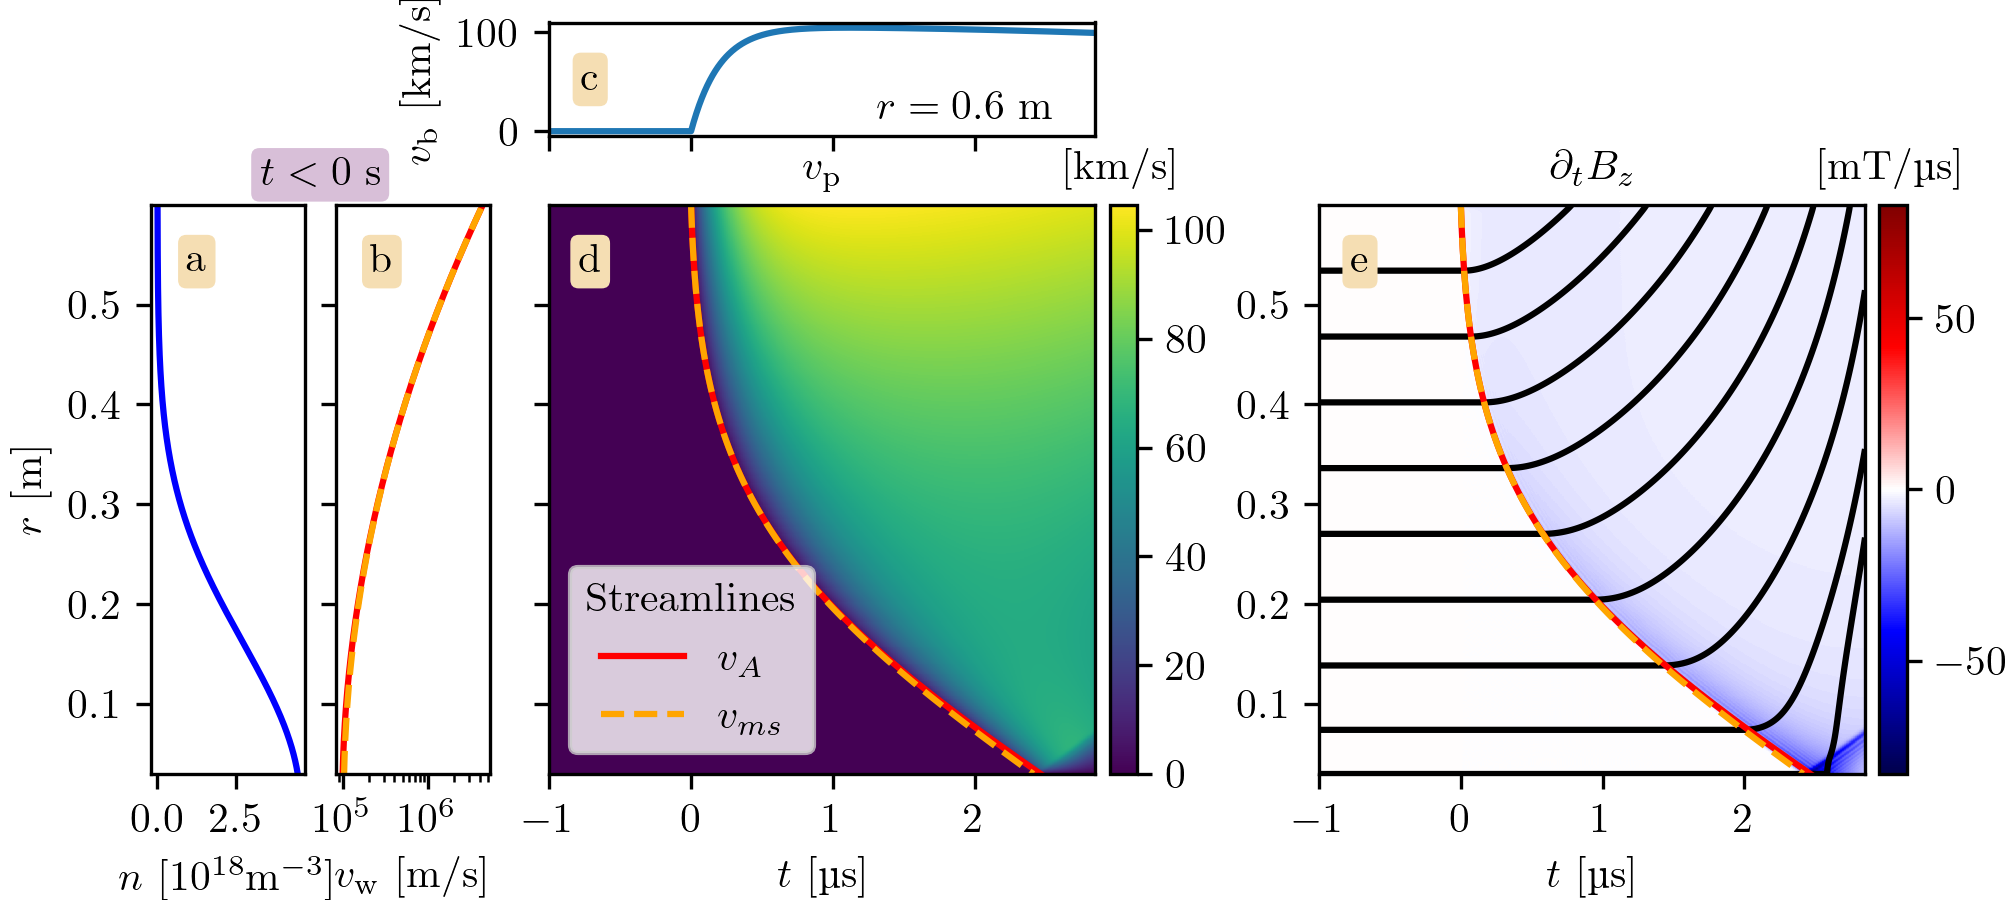
\includegraphics[width=\textwidth]{chapter_pressure_wave/figures/v_and_bdot_w_simulation_setup.png}
    \caption{The simulated wavefront from a 1D linearized MHD simulation. Panel a shows the initial density profile and panel b shows the Alfv\'en speed (red) and fast magnetosonic speed (orange dashed) which are nearly the same. Panel c is the boundary velocity set by the applied loop voltage. Panel d is the velocity of the plasma which only begins to move outward once the wavefront passes with the different speed streamlines drawn on top. Panel e shows the expected measurements from a B-dot coil and flux contours which are similar to \ref{fig:experimental-evolution}, a.}
    \label{fig:simulation-setup}
\end{figure*}

Simulation results can be seen in Fig. \ref{fig:simulation-setup}. Panels a and b show the initial plasma distribution and corresponding wave speeds for the Alfv\'en and fast magnetosonic waves where
\begin{align}
    v_s &\approx \sqrt{\frac{\gamma T_0}{m_i}} \\
    v_A &\approx \frac{B_0}{\sqrt{\mu_0 n_0 m_i}} \\
    v_{ms} &= \sqrt{v_A^2 + v_s^2}.
\end{align}
The propagation angle of the wave relative to the background field is always 90\textdegree. Panel d shows streamlines traveling at $v_A$ and $v_{ms}$ which are very similar for our low beta system. Both streamlines match the speed of the wavefront caused by the initial change in the boundary velocity (panel c). Finally, panel e shows the expected $\partial_t B_z$ signal which matches well with the measured signal from Fig. \ref{fig:experimental-evolution}, panel a.

The $\partial_t B_z$ response is derived from equation \ref{eq:mhd_ohms_faradays_linear_displacement} where we find
\begin{align*}
  \partial_t \bm{B}_1 &= \nabla \times (-B_{z, 0} \partial_t \xi \hat{\phi} + B_{\phi, 0} \partial_t \xi \hat{z}) \\
  \partial_t B_{1, r} &= 0 \\
  \partial_t B_{1, \phi} &= -\partial_r (B_{\phi, 0} \partial_t \xi) \\
  &= - \partial_r B_{\phi, 0} \partial_t \xi - B_{\phi, 0} \partial_{r} \partial_{t} \xi \\
  \partial_t B_{1, z} &= \frac{1}{r} \partial_r (-r B_{z, 0} \partial_t \xi) \\
  &= -\frac{1}{r} B_{z, 0} \partial_t \xi - \partial_r B_{z, 0} \partial_t \xi - B_{z, 0} \partial_{r} \partial_{t} \xi
\end{align*}

We find that the simulation is very similar to the observed B-dot measurements so, assuming that the wave travels at approximately the Alfv\'en speed, we can extract the initial plasma density profile if we know the experimental wave speed.

\section{Experimental Application}

\subsection{Extracting Wave Speed}

\begin{figure}[]
    \centering
    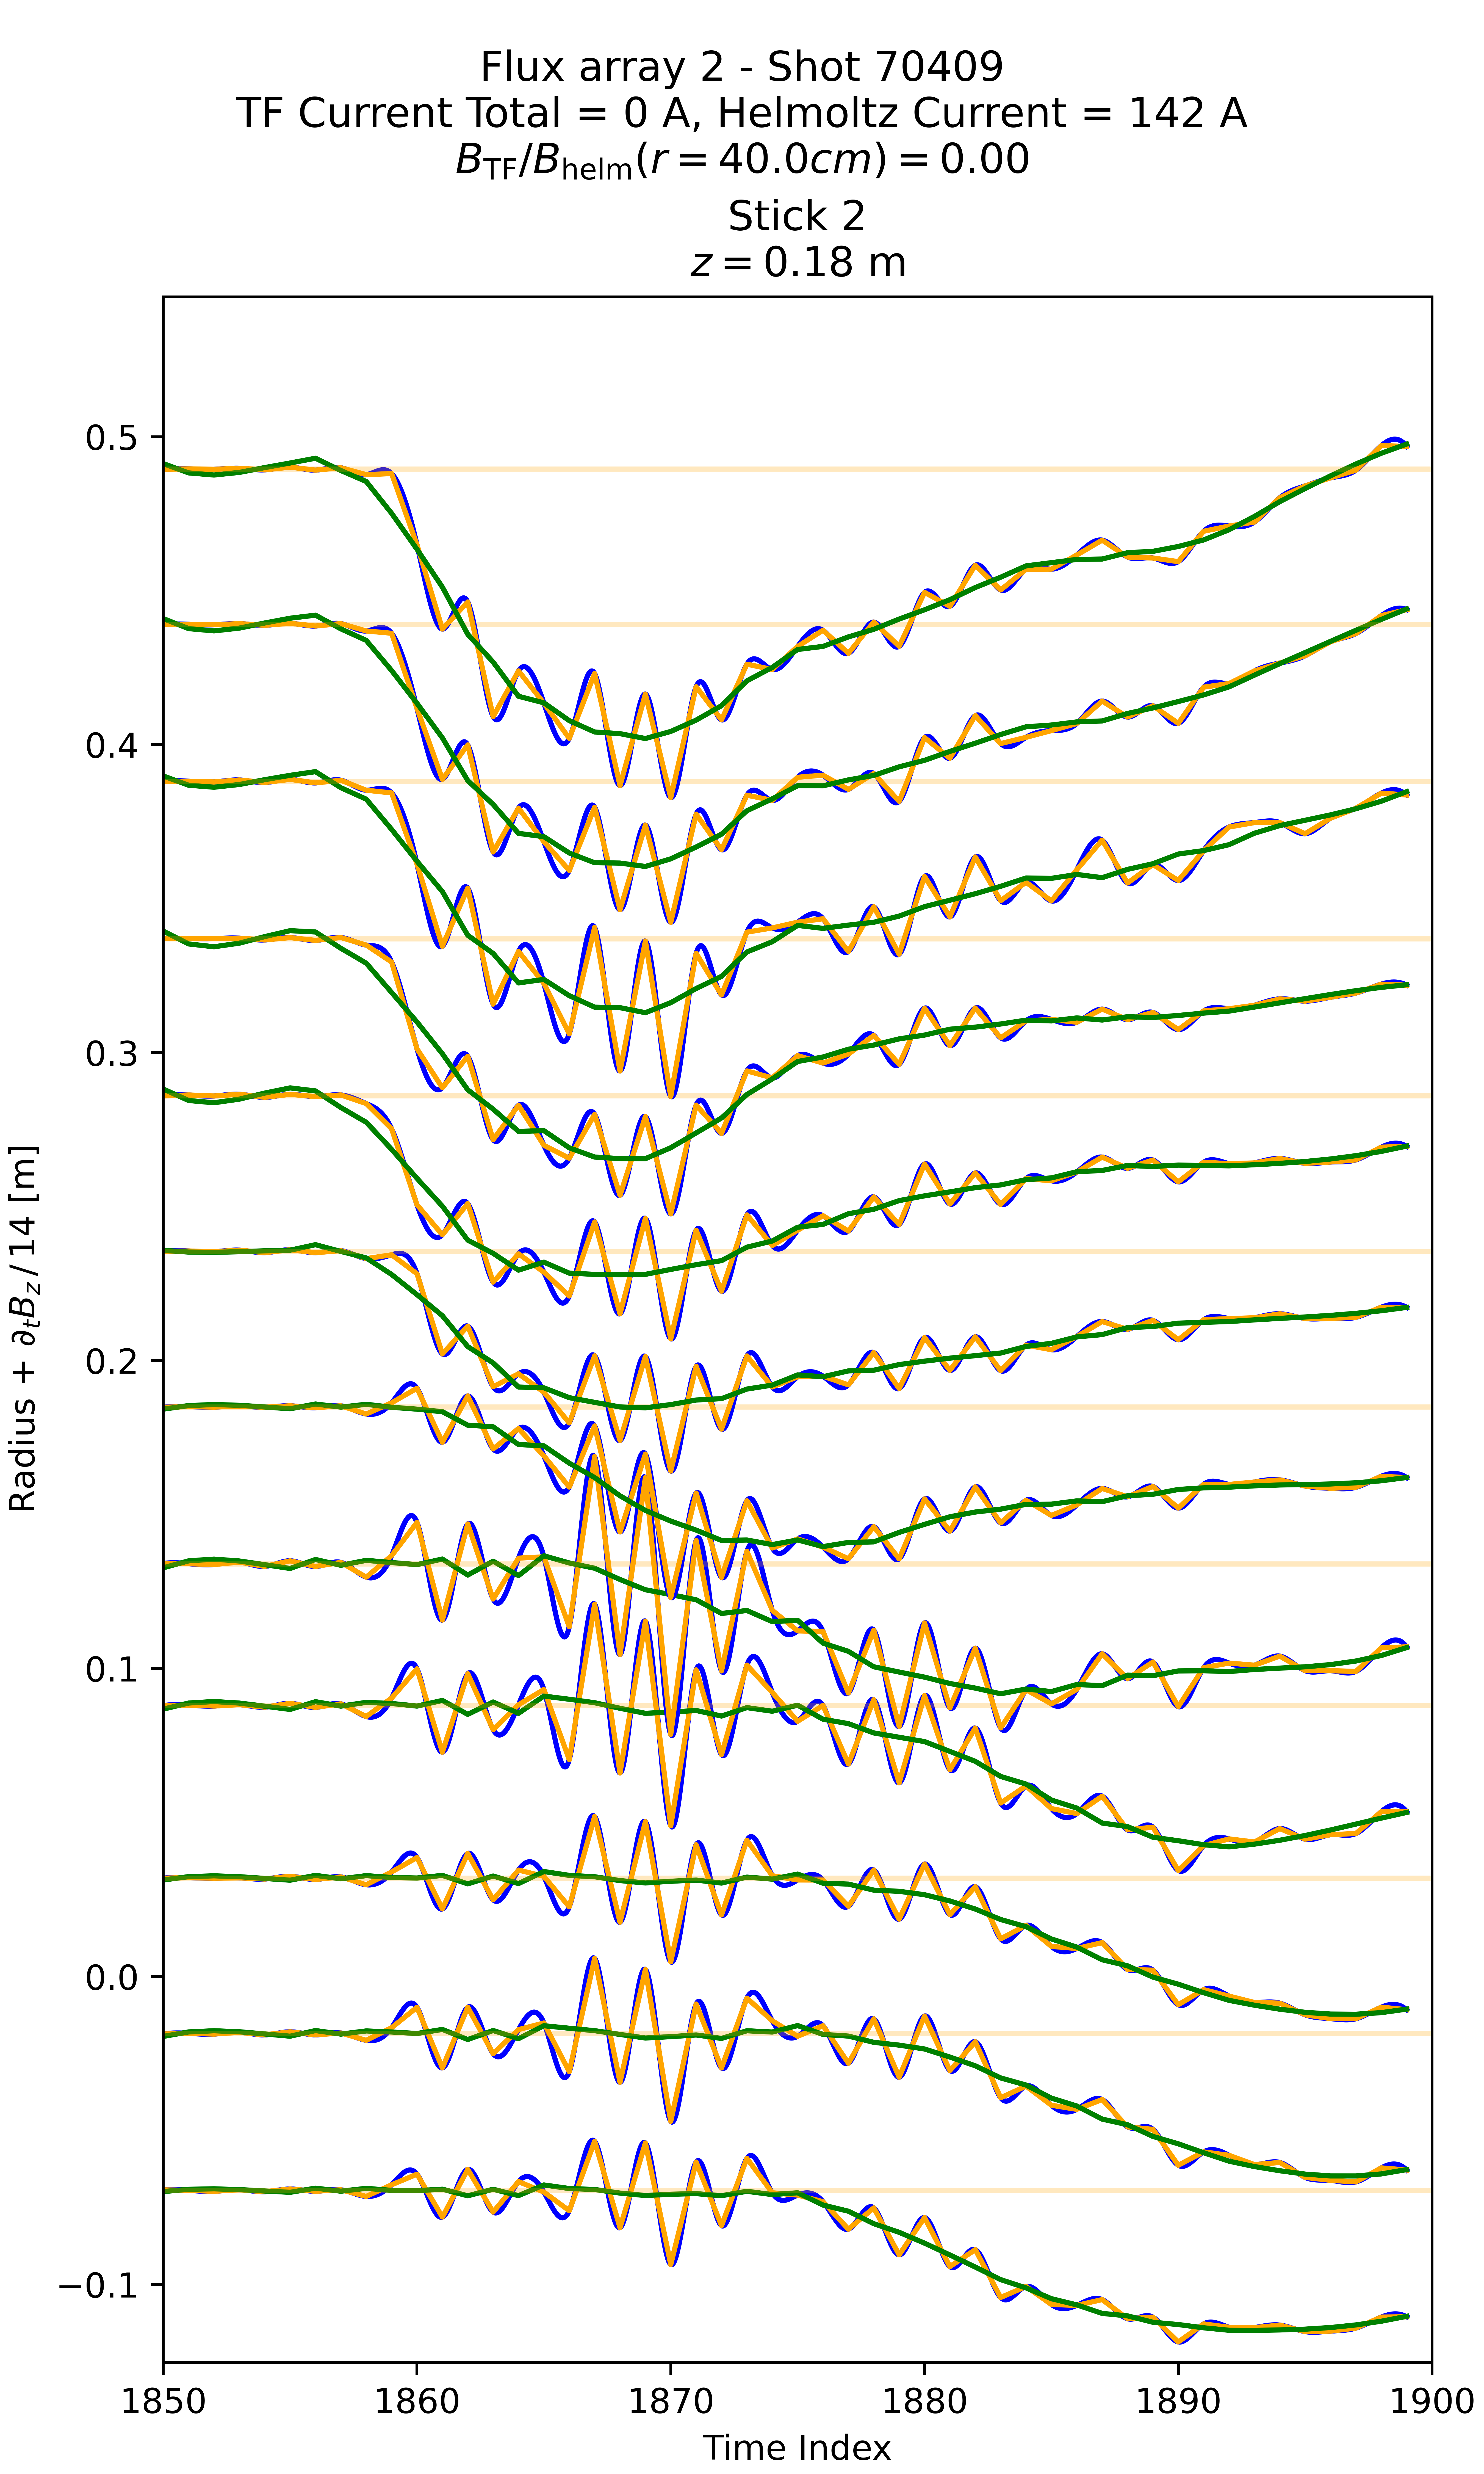
\includegraphics[height=0.8\textheight]{chapter_pressure_wave/figures/example_bdot_traces.png}
    \caption{Experimental measurements of the normalized $\partial_t B_z$ measurements along a radial chord at $z = 18$ cm (the $z$-center of the drive coils is $z = 15$ cm). The radius of each the probe is given by the horizontal pale orange line. Each probe's measurements are normalized and offset to the probes radial location. The orange scatter points are the raw measurements and the blue line that intercepts the scatter points is an interpolation. The blue line has many oscillations that are due to noise in the system. The green smooth line is interpolated data after smoothing using a Savitzky-Golay filter.}
    \label{fig:pressure_wave_raw_bdot_traces}
\end{figure}

We measure the speed of the pressure wave by setting a bounding value for the measured B-dot. When the measured B-dot crosses that threshold we say that the wave has passed the probe. Using the crossing time and probe radius we can calculate the wave speed between two probes.

\subsubsection{Wave tracking}

This very simple thresholding method works but requires some fine tuning to avoid various issues. Figure \ref{fig:pressure_wave_raw_bdot_traces} shows some example B-dot traces from the flux array for a single shot. Here we can see common mode noise (which is very large around time index 1870) exists on all channels and thus the interpolated data (blue) has wild oscillations there. Without some work, the threshold would often set the wave-probe intersection time far earlier than the actual intersection time.

Many of the noisy oscillations can be smoothed out as shown in the green line in figure \ref{fig:pressure_wave_raw_bdot_traces} which show marked improvement over the raw interpolated signal in blue.

To enforce causality, we give the wave some `inertia'. Instead of setting the intersection to the first location where the B-dot signal is greater than the threshold, we decide the time based on the waves previous speed. We start by finding the crossing point for the two probes at the highest radius. Then we calculate $v_0 = \Delta r / \Delta t = (r_1 - r_0) / (t_1 - t_0)$. Using this speed we constrain $t_2$ ($r_2$ having been set by the radius of the probe) as $t_2 > t_1 + C (r_2 - r_1) / v_0$. This forces the wave to keep up some amount of speed which we can determine by choosing $1 \geq C \geq 0$, the inertia factor.

As we decide on both an inertia factor and a B-dot threshold, we can use random choices of these to get an estimate of the wave speed distribution at each radial location. Using a random sampling of these parameter we find a mean and standard distribution for the wave speeds.

\subsection{Getting the density}

Once we have the wave speed it is a simple enough process to extract the plasma density. If we knew the initial temperature profile, we could use the full magnetosonic wave relation but for simplicity and to reduce the need for a temperature measurement, our low beta system sets $v_{ms} \approx v_A$. With our known initial magnetic field which is only slightly perturbed by the plasma we can then solve for $n_0$ finding
\begin{equation}
    n_0 \approx \frac{B_0^2}{\mu_0 m_i v_A^2}
\end{equation}

\subsection{Minimum measurable density}

It can be seen that as the density decreases, the speed of the wave increases and this can lead to resolvability issues where the wave is traveling so quickly that it passes two probes in the time it takes between sample points. A first approximation to this minimum can be written as
\begin{align}
    n_\text{min} &= \frac{B_0^2}{\mu_0 m_i v_{\text{max}}^2} \\
    v_\text{max} &= (r_{i + 1} - r_i) f
\end{align}
where $f = 10$ MHz is the sampling frequency of the digitizer.

We find in practice that this overestimates the minimum measurable density because it assumes that we are limiting the wave crossing time to match with the time sampling. Since we instead find the crossing point of the interpolated data this means we have subsample resolution for our B-dot data so a better approximation derived empirically is
\begin{equation}
    v_\text{max} = (r_{N - 1} - r_0) \frac{f}{2}
\end{equation}
where $N$ is the number of probes.

% \subsubsection{Assuming sample resolution}

% \paragraph{What does this assumption derive}

% \paragraph{How does it compare to the data}

% \paragraph{We need a better approximation}

% \subsubsection{Assuming sub-sample resolution}

% \begin{figure}
%     \caption{Data vs. crude minimum density vs. empirical minimum density}
% \end{figure}

% \subsubsection{A more complex model assuming the plasma is a step function * linear}

% \begin{figure}
%     \caption{Diagram of what the more complex model looks like.}
% \end{figure}

\section{Results}

Since the wave travels at approximately the Alfv\'en speed and we have derived an algorithm for finding the density, we can compare the results of this method to that of a multi-tip Langmuir probe as described in chapter \ref{sch:multitip_probe}.

\subsection{Experimental setup}

A CAD diagram of the experimental setup used for these results can be seen in figure \ref{fig:pressure_wave_brb_cad_rendering}. We measure the magnetic field evolution using the flux arrays which are not shown in the figure but give us density profiles at many different $z$ positions. We find that all of the B-dot signals are similar and thus the assumption of $z$ symmetry is accurate. We insert the multi-tip Langmuir probe into a port on the equator such that it passes between the two halves of the drive cylinder and measures along a radial chord.

\begin{figure}
    \centering
    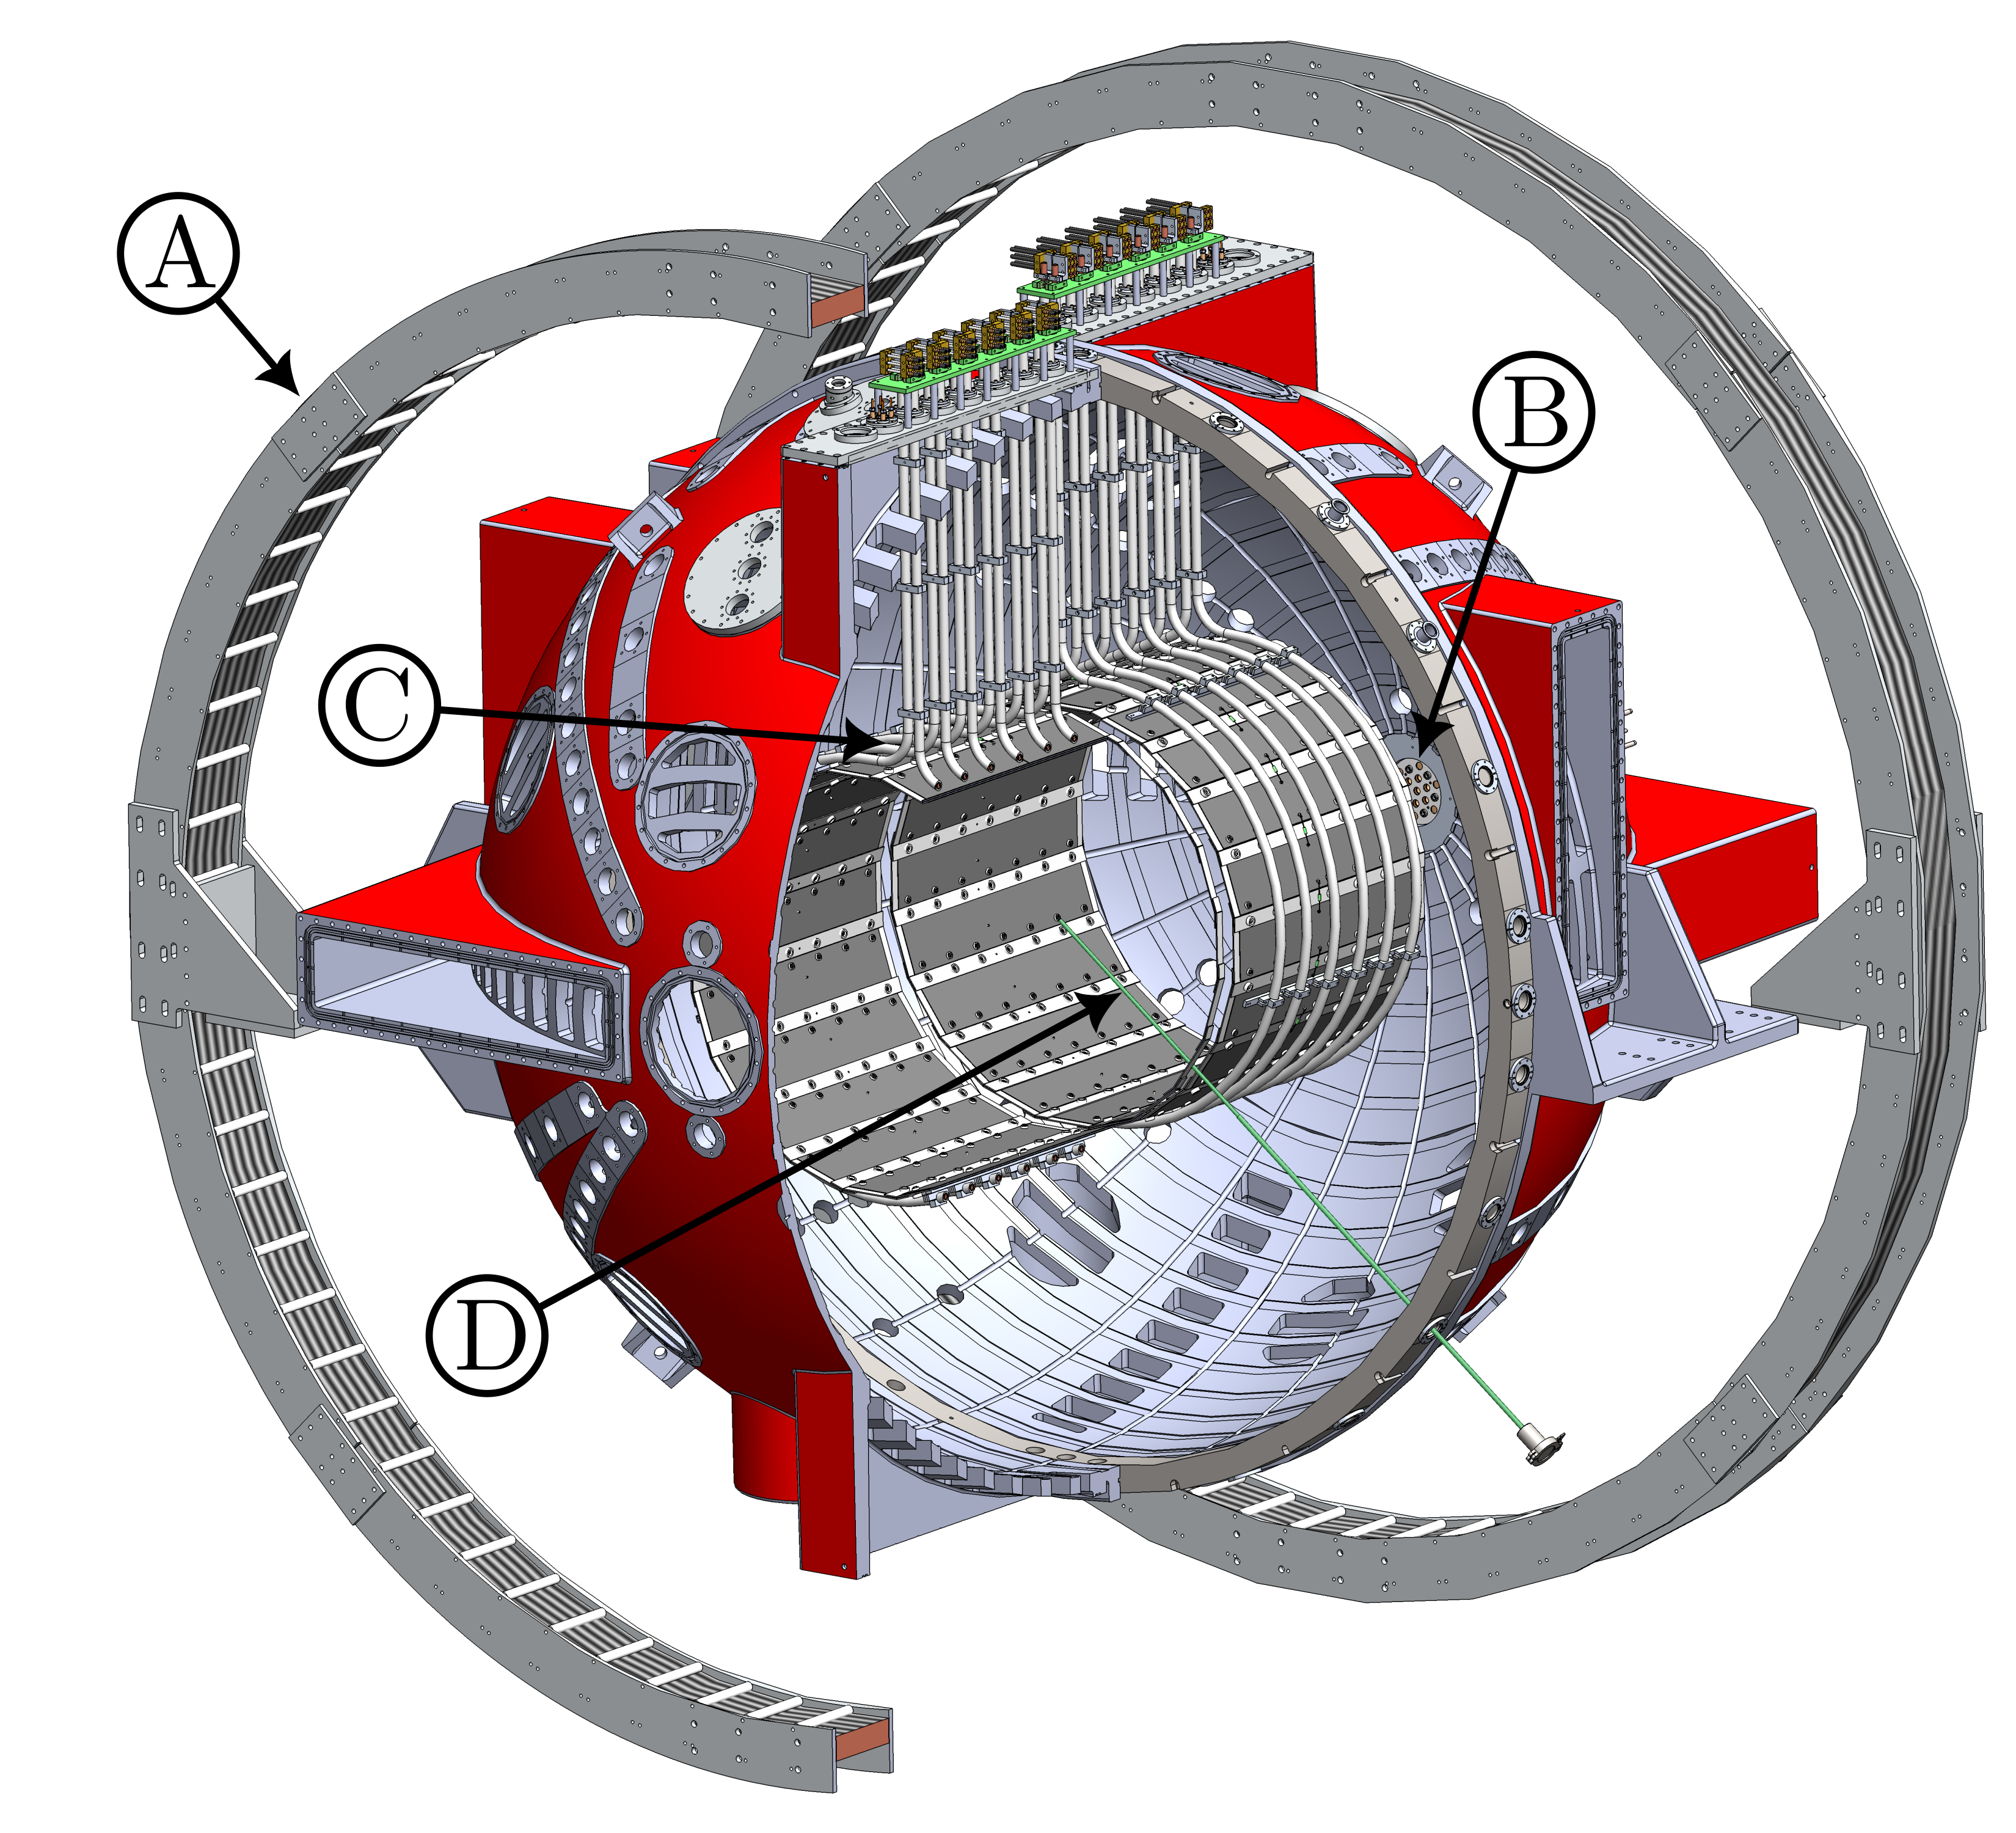
\includegraphics{chapter_pressure_wave/figures/brb_cad_drive_cylinder.png}
    \caption{A CAD rendering of the BRB with the drive cylinder. The background $z$ field is set by the Helmholtz coil (A) and plasma is injected from plasma guns near $r = 0$ (B). After the plasma has equilibrated in the machine, a reversed field is driven by the drive cylinder (C) and the evolution of the magnetic field is done by arrays of B-dot probes on radial chords or at a single location per shot by a multi-tip Langmuir probe (D).}
    \label{fig:pressure_wave_brb_cad_rendering}
\end{figure}

\subsection{Langmuir vs. Pressure Wave Results}

\begin{figure}
    \centering
    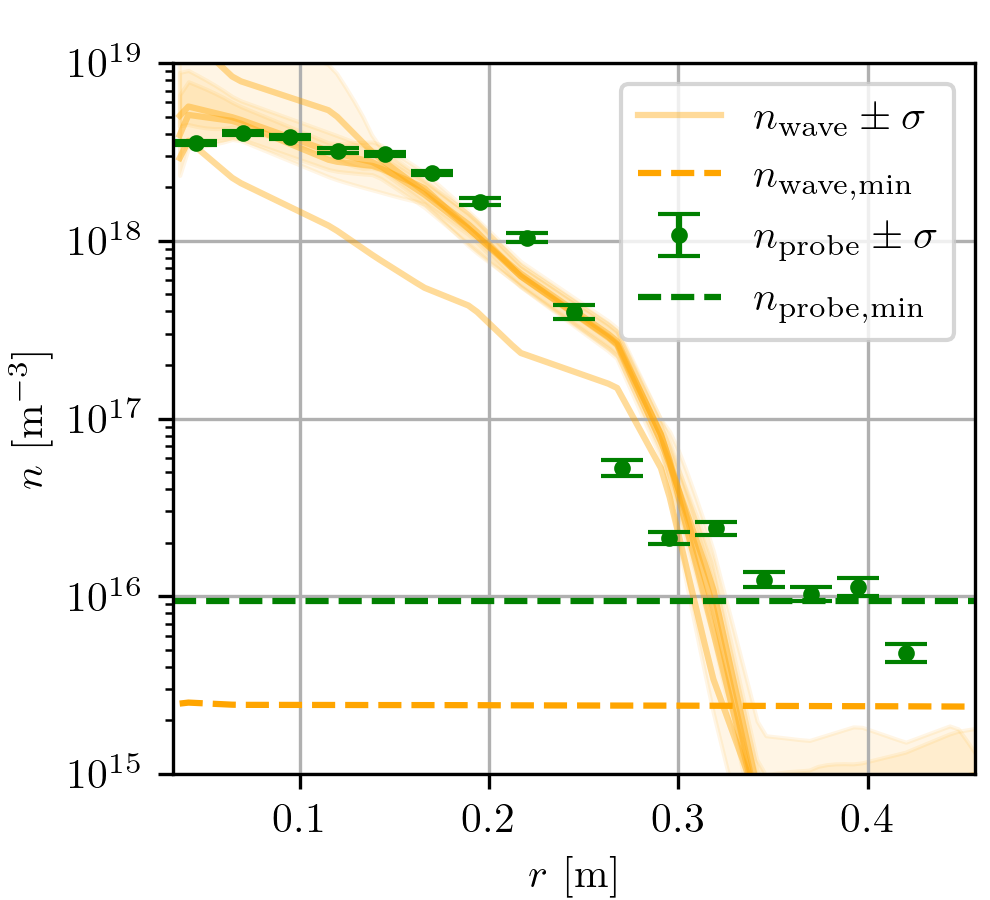
\includegraphics{chapter_pressure_wave/figures/wave_density_vs_probe_density.png}
    \caption{Plot of the initial plasma density measured by the Langmuir probe and pressure wave. The solid orange lines are measurements from different shots with filled area around each line setting the standard deviation. It can be seen that one shot can be easily identified as an outlier with exceptionally low density at low radii. The orange dashed line sets the minimum measurable density for the pressure wave. The green scatter points are measurements from the Langmuir probe with minimum density described in \ref{sss:multitip_min_density}.}
    \label{fig:pressure_wave_langmuir_vs_wave_density}
\end{figure}

Figure \ref{fig:pressure_wave_langmuir_vs_wave_density} shows a comparison between measurements of the initial plasma density using the Langmuir probe over many shots (each point in the plot being a separate shot) and the pressure wave profiles (each profile is a single shot). The advantage of the pressure wave method is that each shot fully reproduces the radial density profile (for $N$ B-dot coils it would take $N$ shots with the Langmuir probe to get the same result).

It can be noted that the Langmuir probe and the pressure wave show very similar trends except when the probe is nearing it's minimum measurable density. Additionally, we have used the pressure wave as absolute calibration of the Langmuir probe area so the scaling of the scatter points is set after the fact.

\subsection{Wave Evolution}

As we have the entire simulated evolution of the magnetic field, we can compare the experimental measurements of figure \ref{fig:pressure_wave_raw_bdot_traces} to that simulated in figure \ref{fig:pressure_wave_simulated_bdot_trace}. We see that in the simulation, high frequency modes grow as the wave moves radially inwards whereas the wave smooths as it propagates from experimental results.

We believe that the cause of this may be from two-fluid effects where the ions and electrons decouple at a high enough frequency such that the wave speed shifts. Additionally, there may be some dissipation of the wave energy and lack of cylindrical symmetry that lead to a smoothing of high frequency and a decrease in wave amplitude.

\begin{figure}
    \centering
    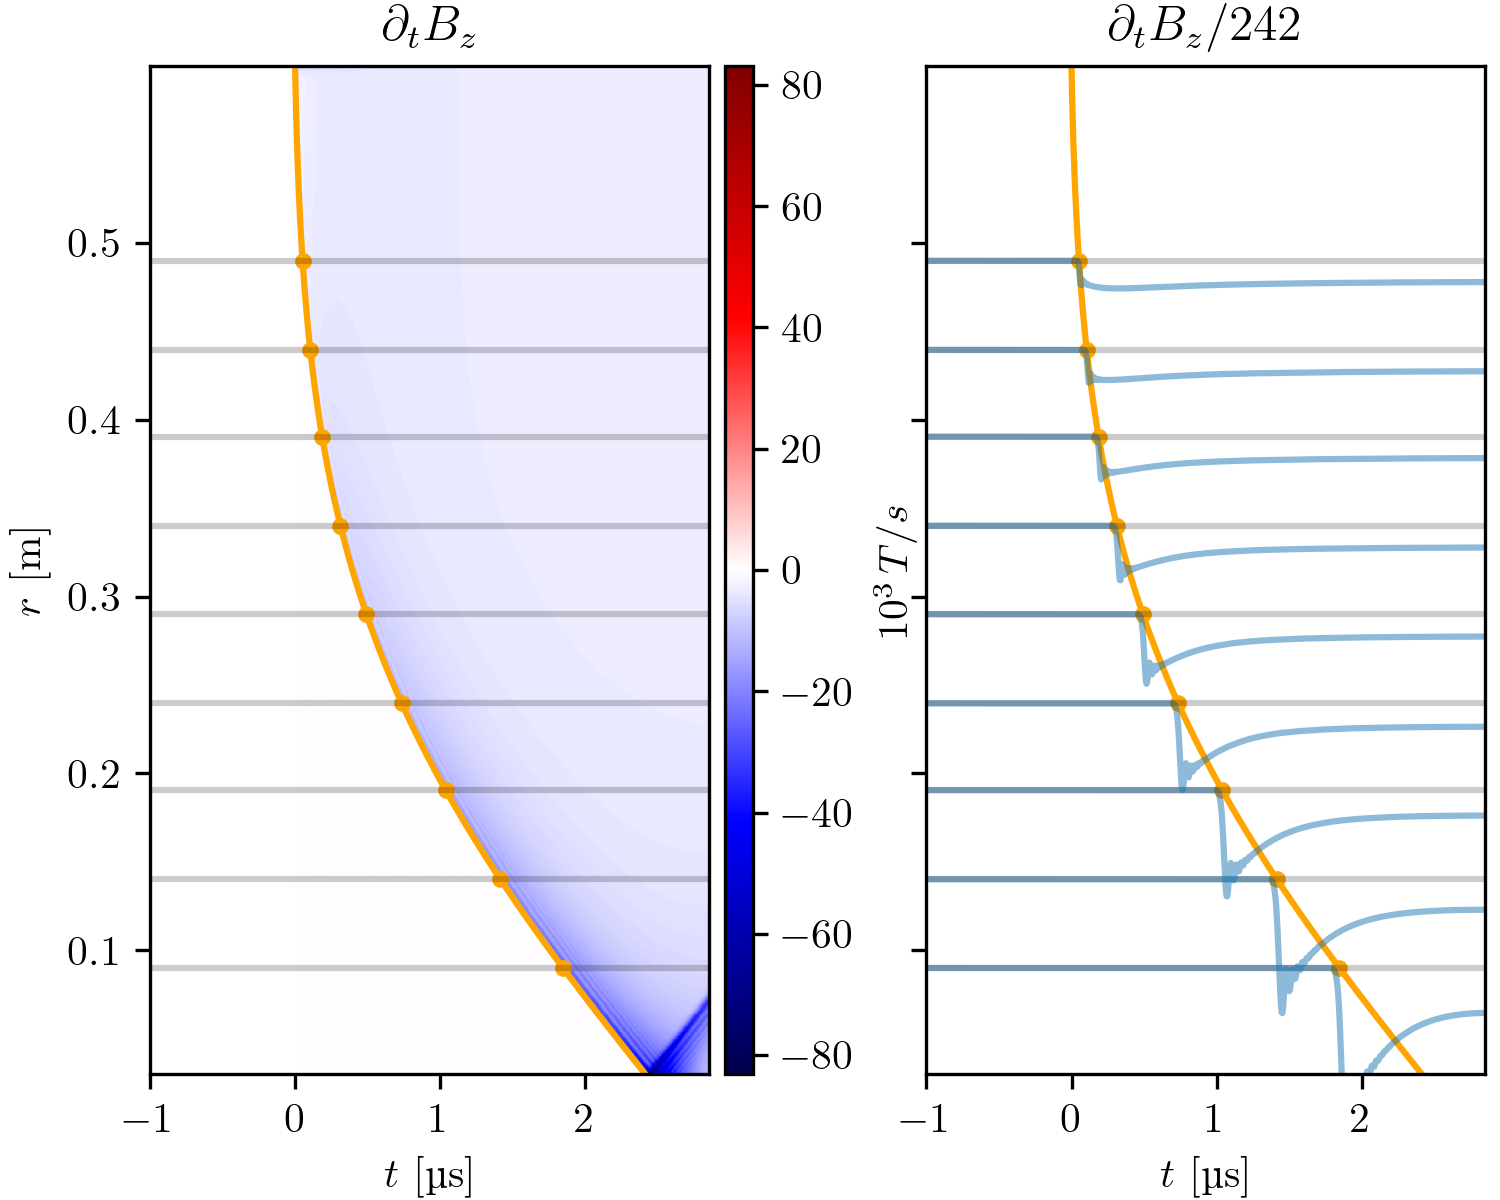
\includegraphics{chapter_pressure_wave/figures/bdot_w_r_cuts.png}
    \caption{The left plot shows the expected magnetic field evolution from the simulation and the right plot shows the evolution of $\partial_t B_z$ in time for a variety of radii which are in positions similar to figure \ref{fig:pressure_wave_raw_bdot_traces}. The orange line shows the wavefront with orange dots being the points where the wave crosses the radial position. The right panel shows the growth of high frequency modes in the wavefront.}
    \label{fig:pressure_wave_simulated_bdot_trace}
\end{figure}

To study the possible two-fluid effects we plot the dispersion relation in figure \ref{fig:pressure_wave_two_fluid_dispersion} as derived by \cite{Bellan_2012} and implemented in \cite{PlasmaPy}. It can be seen that the high frequency components of the wavefront are expected to move slower as compared to frequencies below the MHD cutoff, which for the given parameters is $\approx 9 \cdot 10^5$ Hz.

\begin{figure}
    \centering
    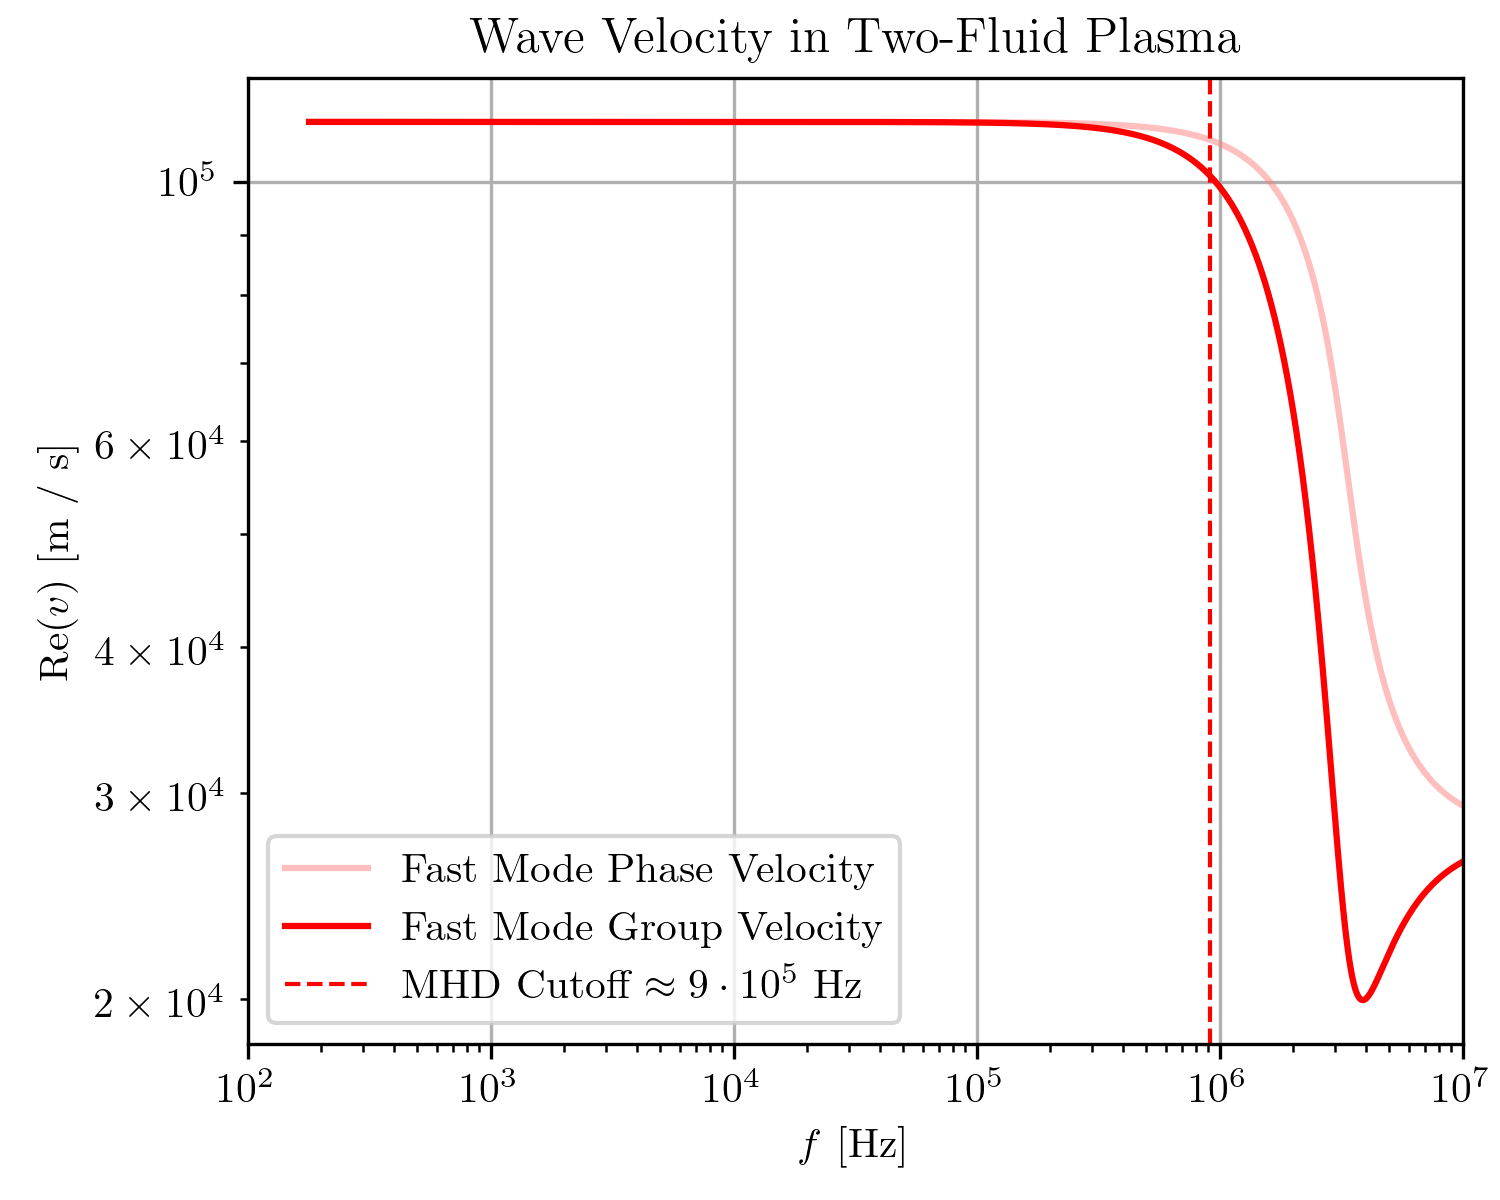
\includegraphics{chapter_pressure_wave/figures/two_fluid_velocity.png}
    \caption{The phase and group velocities for the fast magnetosonic wave as a function of frequency. The MHD cutoff is set to when the phase velocity differs by more than 10\% of the fast magnetosonic speed derived from MHD. The plasma parameters here are $n = 10^{18}$ m$^{-3}$, $B = 5$ mT, $T_e = 5$ eV, $T_i = 1$ eV, and propagation angle $\theta = 90^\circ$.}
    \label{fig:pressure_wave_two_fluid_dispersion}
\end{figure}

This means that high frequency components will be delayed and the wavefront should smooth as it propagates inwards which is what we see in figure \ref{fig:pressure_wave_raw_bdot_traces}. The dispersion relation does not illuminate the dissipative effects that may decrease the high frequency amplitudes which are still unexplained in our experiment.

% TODO: Add simulation results if I have any.
% \paragraph{How to simulate evolution approximately}

% \paragraph{Dispersion simulation results}

% \begin{figure}
%     \caption{Results of simulating application of dispersion relation to pressure wave}
% \end{figure}

% TODO: Figure out if I should talk about this applications stuff.
% \section{Applications}

% \subsection{System Requirements}

% \subsubsection{Cylindrical symmetry}

% \subsubsection{Releasing magnetic pressure at high radius}

% \subsubsection{Measurements along a radial chord}

% \subsubsection{Known initial field}

% \subsection{Other Machines}

% LAPD \& MRX

% \subsection{Diagnosing Gun failures}

% \begin{figure}
%     \caption{Initial density before and after many shots}
% \end{figure}

% \subsection{Measuring effect of different gun number and Helmholtz strength}

% \subsubsection{Gun number}

% \begin{figure}
%     \caption{Initial density for varying gun number}
% \end{figure}

% \subsubsection{Helmholtz}

% \begin{figure}
%     \caption{Initial density for varying Helmholtz}
% \end{figure}

% \subsection{Measuring diffusion coefficient}

% \subsubsection{Diffusion theoretical model}

% \begin{figure}
%     \caption{Diagram of flux mechanisms.}
% \end{figure}

% \subsubsection{Diffusion simulations}

% \begin{figure}
%     \caption{Example diffusion simulation}
% \end{figure}

% \subsubsection{Applications of pressure wave model}

% I think I need to do a bit more research here to show that we can actually extract a diffusion coefficient.

% TODO: What all should I include in this section?
\section{Future Research}

\subsection{Better wave tracking}

There are a number of potential improvements in estimating the wave speed. With these advances, constraints on the density between probe measurements could be made along with better error accounting.

\subsubsection{Cross-correlation and Dynamic Time Warping}

The current method for tracking the wave involves finding when the B-dot signal is larger than some value. Unfortunately this only uses two data points from a coil to find the wave crossing time and thus will be very sensitive to noise (which is especially prominent because of the capacitor bank switching). To avoid this issue via multi-point analysis, tracking could use either of the following algorithms:

\paragraph{Cross-Correlation} This method operates by comparing each signal, $\vb{S}_i(t)$, against the next, $\vb{S}_{i + 1}(t)$ via
\begin{equation}
    C_{i, i + 1}(\Delta t) = \int \vb{S}_i(t) \cdot \vb{S}_{i+1}(t + \Delta t) \dd{t}
\end{equation}
which can be extended into a discrete formulation (which we'll leave for the reader). It can be seen that if $\vb{S}_{i + 1}(t) = \vb{S}_{i}(t + A)$ then $\max_{\Delta t} C_{i, i + 1}(\Delta t) = C_{i, i + 1}(A)$. A method using an integral of a subset of the signal could work out to better line up when the wave hits probes at different locations and there may be ways to use a full correlation matrix of $C_{i,j}$ to better constrain the wave timing and avoid noise.
% \begin{figure}
%     \caption{Example of cross-correlation}
% \end{figure}


\paragraph{Dynamic Time Warping (DTW)} This algorithm has some similarities to cross-correlation but is a little fancier. It takes two signals and finds how much to shift each data point in time to make them best align with an example shown in figure \ref{fig:wave_dtw}. This has the ability to track multiple features during the pressure wave (such as oscillations of the signal due to transmission line effects as seen in section A.6 of \cite{Gradney_2025}) which could measure the evolution of the density profile. The algorithm calculates a loss function where measurements that are far apart are avoided and a path from the first time point to the last point is found that minimizes the loss (red line in \ref{fig:wave_dtw}). The distance the line is away from no time index offset (green dashed line) is the time delay between the signals for that feature in the signal.
\begin{figure}
    \centering
    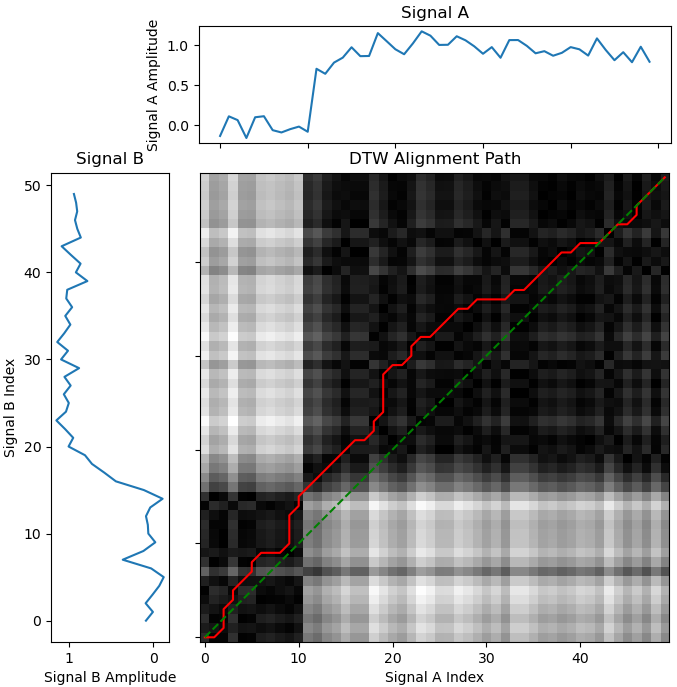
\includegraphics[width=\textwidth]{chapter_pressure_wave/figures/dtw_example.png}
    \caption{Example of DTW}
    \label{fig:wave_dtw}
    % TODO: Expand this caption.
\end{figure}

\subsubsection{Modeling Wave Evolution}

It can be seen by comparing figure \ref{fig:pressure_wave_simulated_bdot_trace} and \ref{fig:pressure_wave_raw_bdot_traces} that the simulation does not match the experimental measurements in terms of the evolution of the wave. Modeling the wave evolution based on the two-fluid dispersion relation may give some more insight into these differences and may also help to find when the wave hits a probe.

\subsection{Fast-Magnetosonic Speed}

If, instead of using the Alfv\'en speed, the fast magnetosonic speed were to be used, a more accurate density measurement could result. Unfortunately this relies on the initial plasma temperature which may or may not be uniform. Accurate modeling of the initial temperature distribution and the effects of cool ions would result in a more accurate density measurement.

\subsection{Cross-field Diffusion}

The pressure wave density profile lets us quickly extract the full density profile for a given initial equilibrium. By doing so we could use it for estimating what processes the plasma undergoes to diffuse outwards from the center field lines where it is injected out to high radii. Taking shots with variable Helmholtz field and toroidal field would give different field distributions and by modeling losses to the wall and outward diffusion, the diffusion coefficients dependence on magnetic field and density could be measured.
